\section{Der Datensatz}
arXiv.org ist ein Dokumentenserver f�r Preprints aus dem Bereich der naturwissenschaftlichen F�cher. Ver�ffentlichungen k�nnen ohne Begutachtung auf dem Server abgelegt werden und werden nach dem Open-Access-Prinzip f�r jedem kostenfrei zur Verf�gung gestellt.

Der von uns verwendete Datensatz liegt im XML-Format vor und benutzt ein von der Dublin Core Initiative \footnote{http://dublincore.org/} spezifiziertes Schema.
Jeder Eintrag f�r eine Publikation wird von einem \PY{n+nt}{<record}\PY{n+nt}{>} Tag umschlossen und alle Eintr�ge werden in \PY{n+nt}{<ListRecords}\PY{n+nt}{>} aufgef�hrt.
\begin{program}
\begin{Verbatim}[commandchars=\\\{\}, fontsize=\footnotesize, frame=single]
\PY{c+cp}{<?xml version="1.0" encoding="UTF-8"?>}
\PY{n+nt}{<OAI-PMH} \PY{n+na}{xmlns=}\PY{l+s}{"http://www.openarchives.org/OAI/2.0/"}
  \PY{n+na}{xmlns:xsi=}\PY{l+s}{"http://www.w3.org/2001/XMLSchema-instance"} 
  \PY{n+na}{xsi:schemaLocation=}\PY{l+s}{"http://www.openarchives.org/OAI/2.0/OAI-PMH.xsd"}\PY{n+nt}{>}
  \PY{n+nt}{<responseDate}\PY{n+nt}{>}
    2011-10-05T16:49:31Z
  \PY{n+nt}{</responseDate>}
  \PY{n+nt}{<request} \PY{n+na}{verb=}\PY{l+s}{"ListRecords"} \PY{n+na}{metadataPrefix=}\PY{l+s}{"oai\PYZus{}dc"}\PY{n+nt}{>}
    http://export.arxiv.org/oai2
  \PY{n+nt}{</request>}
    \PY{n+nt}{<ListRecords}\PY{n+nt}{>}
      \PY{n+nt}{<record}\PY{n+nt}{>}
        \PY{n+nt}{<header}\PY{n+nt}{>}
          ...
        \PY{n+nt}{</header>}
        \PY{n+nt}{<metadata}\PY{n+nt}{>}
          ...
        \PY{n+nt}{</metadata>}
      \PY{n+nt}{</record>}
        ...
      \PY{n+nt}{<record}\PY{n+nt}{>}
        \PY{n+nt}{<header}\PY{n+nt}{>}
          ...
        \PY{n+nt}{</header>}
        \PY{n+nt}{<metadata}\PY{n+nt}{>}
          ...
        \PY{n+nt}{</metadata>}
      \PY{n+nt}{</record>}
    \PY{n+nt}{</ListRecords>}
\PY{n+nt}{</OAI-PMH>}
\end{Verbatim}

\caption{Struktur des Datensatzes}
\end{program}
\subsection{Aufbau der Eintr�ge}
Jeder Eintrag setzt sich aus zwei Teilen zusammen: den \PY{n+nt}{<header}\PY{n+nt}{>} und \PY{n+nt}{<metadata}\PY{n+nt}{>} Teil.
\subsubsection{Header}
Im Header-Teil eines Eintrages sind arXiv-spezifische Informationen zur jeder Publikation zu finden.
Der \PY{n+nt}{<identifier}\PY{n+nt}{>} ist ein eindeutiger Bezeichner f�r eine Publikation in der arXiv-Datenbank.
Das \PY{n+nt}{<datestamp}\PY{n+nt}{>} Attribut enth�lt das Datum der letzten Bearbeitung des Eintrags auf dem arXiv-Server.
Die \PY{n+nt}{<setSpec}\PY{n+nt}{>} Attribute enthalten die von arXiv zugeordneten Themen f�r eine Publikation.
\begin{program}
\begin{Verbatim}[commandchars=\\\{\}, fontsize=\tiny, frame=single]
\PY{n+nt}{<identifier}\PY{n+nt}{>}oai:arXiv.org:0704.0001\PY{n+nt}{</identifier>}
\PY{n+nt}{<datestamp}\PY{n+nt}{>}2007-07-24\PY{n+nt}{</datestamp>}
\PY{n+nt}{<setSpec}\PY{n+nt}{>}\textcolor{red}{\bf{physics:physics}}\PY{n+nt}{</setSpec>}
\PY{n+nt}{<setSpec}\PY{n+nt}{>}\textcolor{red}{\bf{math}}\PY{n+nt}{</setSpec>}
\end{Verbatim}

\caption{Kopfteil eines Eintrages}
\end{program}

\subsubsection{Metadaten}
 In den Metadaten befinden sich alle anderen relevanten Informationen zu einer Publikation.
 Dazu geh�ren z.B. der Titel der Publikation, die Autoren, sowie die Themen.
 Themen werden anhand unterschiedlicher Klassifizierungen vergeben.
 Es werden sowohl arXiv-spezifische Themen vergeben als auch Themen, die auf standartisierten Klassifizierungen, zum Beispiel der ACM-Klassifizierung\footnote{http://www.acm.org/about/class/ccs98-html} oder der MSC-Klassifizierung\footnote{http://msc2010.org/mscwiki/index.php?title=MSC2010}, beruhen.
 Zu jedem Eintrag einer Publikation geh�rt au�erdem ein Abstract, der den Inhalt kurz erl�utern soll.
 Anschlie�end gibt es ein oder mehrere \PY{n+nt}{<date}\PY{n+nt}{>} Attribute, die das Datum aller Ver�nderungen an dem Eintrag der Publikation aufzeichnen.
 Am Ende befinden sich verschiedene eindeutige Bezeichner, um die Publikation in verschiedenen Datenbanken wieder zu finden.
\begin{program}
\begin{Verbatim}[commandchars=\\\{\}, fontsize=\tiny, frame=single]
\PY{n+nt}{<dc:title}\PY{n+nt}{>}Titel des Papers\PY{n+nt}{</dc:title>}
\PY{n+nt}{<dc:creator}\PY{n+nt}{>}Author 1\PY{n+nt}{</dc:creator>}
\PY{n+nt}{<dc:creator}\PY{n+nt}{>}Author 2\PY{n+nt}{</dc:creator>}
\PY{n+nt}{<dc:subject}\PY{n+nt}{>}\textcolor{red}{\bf{Physics - Optics}}\PY{n+nt}{</dc:subject>}
\PY{n+nt}{<dc:subject}\PY{n+nt}{>}\textcolor{red}{\bf{Mathematics - Combinatorics}}\PY{n+nt}{</dc:subject>}
\PY{n+nt}{<dc:description}\PY{n+nt}{>}Description\PY{n+nt}{</dc:description>}
\PY{n+nt}{<dc:description}\PY{n+nt}{>}Comment\PY{n+nt}{</dc:description>}
\PY{n+nt}{<dc:date}\PY{n+nt}{>}\textcolor{red}{\bf{2007-04-02}}\PY{n+nt}{</dc:date>}
\PY{n+nt}{<dc:date}\PY{n+nt}{>}\textcolor{red}{\bf{2007-07-24}}\PY{n+nt}{</dc:date>}
\PY{n+nt}{<dc:type}\PY{n+nt}{>}text\PY{n+nt}{</dc:type>}
\PY{n+nt}{<dc:identifier}\PY{n+nt}{>}http://arxiv.org/abs/0704.0001\PY{n+nt}{</dc:identifier>}
\PY{n+nt}{<dc:identifier}\PY{n+nt}{>}Phys.Rev.D76:013009,2007\PY{n+nt}{</dc:identifier>}
\end{Verbatim}

\caption{Metadaten eines Eintrages}
\end{program}

\subsection{Eigenschaften}
Der Datensatz besteht aus $706\,077$ Eintr�gen mit wissenschaftlichen Publikationen.
Die Publikationen werden im Header-Teil eines Eintrags in 18 Themen (hier Oberthemen genannt) eingeteilt.
Eine Publikation kann ein oder mehrere Themen haben. Die n�chste Abbildung stellt eine Verteilung der Themen im Gesamtdatensatz dar.\\
\begin{figure}[H]
	\centering
	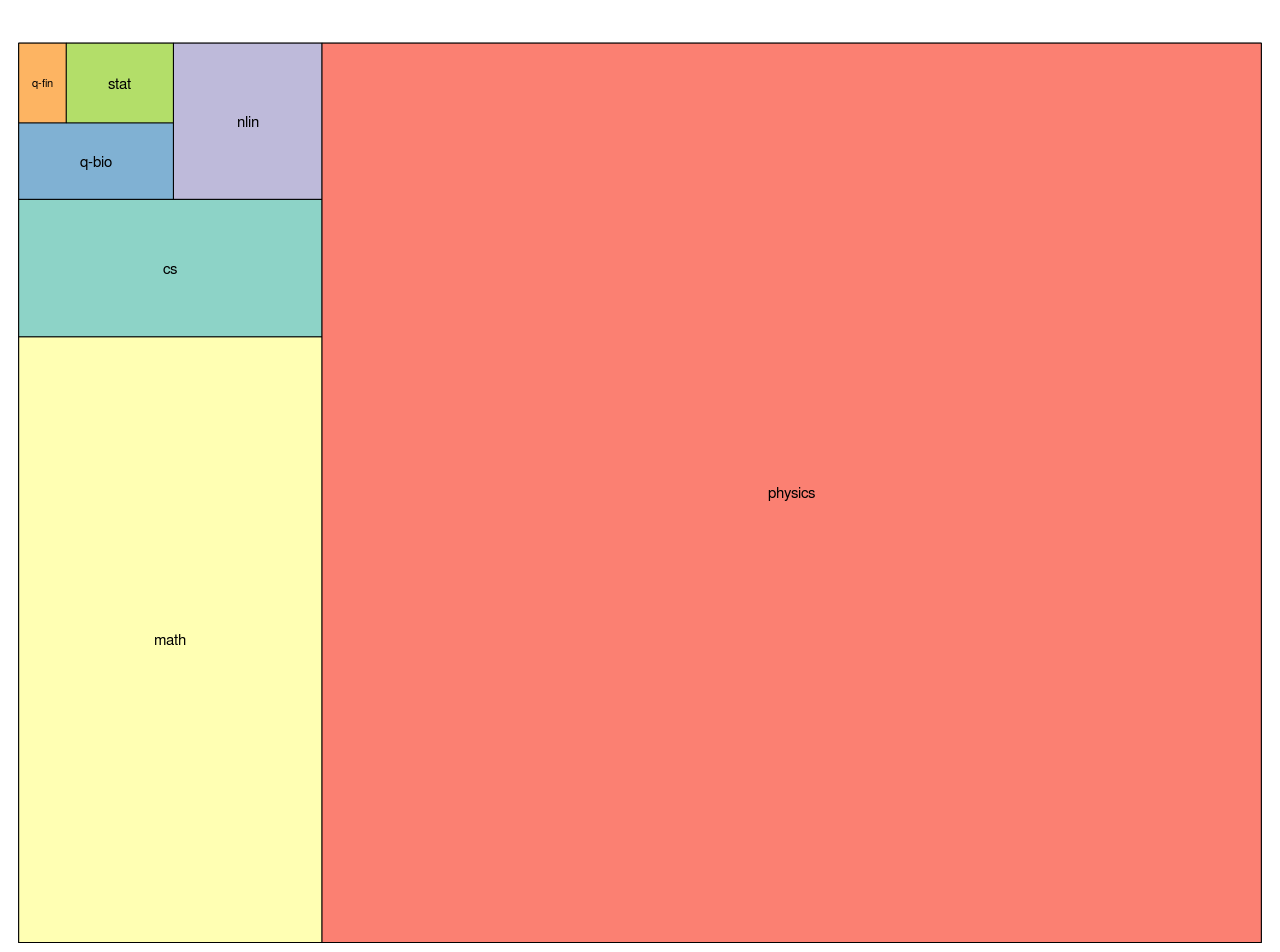
\includegraphics[scale=0.25]{../visual/treemap_no_title.png}
	\caption{Verteilung der Oberthemen im arXiv Datensatz}
	\label{treemap}
\end{figure}

\begin{table}[H]
\centering % used for centering table
\begin{tabular}{| l | l | l |}
	\hline
	Thema & Abk�rzung & Anteil(ca.) \\
	\hline
	Mathematics & math & $21.2 \%$ \\
	Condensed Matter & physics:cond-mat & $20.0 \%$\\
	Astrophysics & physics:astro-ph & $20.0\%$\\
	High Energy Physics - Phenomenology & physics:hep-ph & $13.0\%$\\
	High Energy Physics - Theory & physics:hep-th & $11.7\%$\\
	Physics & physics:physics & $6.8\%$\\
	Quantum Physics & physics:quant-ph &$6.3\%$\\
	General Relativity and Quantum Cosmology & physics:gr-qc & $6.0 \%$\\
	Computer Science & cs & $4.8 \%$ \\
	Mathematical Physics & physics:math-ph & $3.9 \%$\\
	Nuclear Experiment & physics:nucl-th & $3.8\%$\\
	High Energy Physics - Experiment & physics:hep-ex & $2.7\%$\\
	Nonlinear Sciences & nlin &  $2.7 \%$\\
	High Energy Physics - Lattice & physics:hep-lat & $2.1\%$\\
	Quantitative Biology & q-bio &$1.4 \%$ \\
	Nuclear Theory & physics:nucl-ex & $1.3\%$\\
	Statistics & stat & $1.0 \%$ \\
	Quantitative Finance & q-fin & $0.4\%$ \\
	Physics & physics & $0.0 \%$\\
	\hline
\end{tabular}
\caption{Detaillierte Aufteilung der Oberthemen im  Datensatz} % title of Table
\end{table}
Die durschnittliche Anzahl der vergebenen Oberthemen betr�gt $1.3$ und die maximale Anzahl von Oberthemen f�r eine Publikation ist $9$.
Bei rund $80 \%$ aller Publikationen wurde nur $1$ Oberthema im Kopfbereich eines Eintrages vergeben. Bei $14 \%$ aller Themen wurden 2 und bei den restlichen $6 \%$ mehr als 2 Themen vergeben.


\subsection{Eigenschaften vom Thema Computer Science}
Zus�tzlich sollen alle Eintr�ge mit \textbf{cs} als Oberthema betrachtet werden und deren Themen im metadata-Teil untersucht werden.
Die Anzahl der wissenschaftlichen Publikationen mit dem Oberthema \textbf{cs} (Computer Science) betr�gt rund $34\;000$.
Die Bezeichnungen der Themen teilen sich in 2 gro�e Themengruppen auf.
Einerseits werden den Publikationen informatische und mathematische Klassen der Klassifikationsysteme ACM und MSC vergeben, was rund $30 \%$ der Informatikpublikationen betrifft, und andererseits wird eine hierarchische Unterteilung von arXiv.org verwendet, die aus $146$ Bezeichnern der Form ``Fachgebiet - Themengebiet'' z.B. ``Computer Science - Information Theroy'' besteht.
Die durschnittliche Anzahl von Themen pro Eintrag betr�gt hier $2.2$, was, unterm anderen, ein Indikator daf�r ist, dass es sinnvoller ist, Assoziationsregeln der Form $A \rightarrow B$ in den Metadaten zu suchen.
\begin{figure}[H]
	\centering
	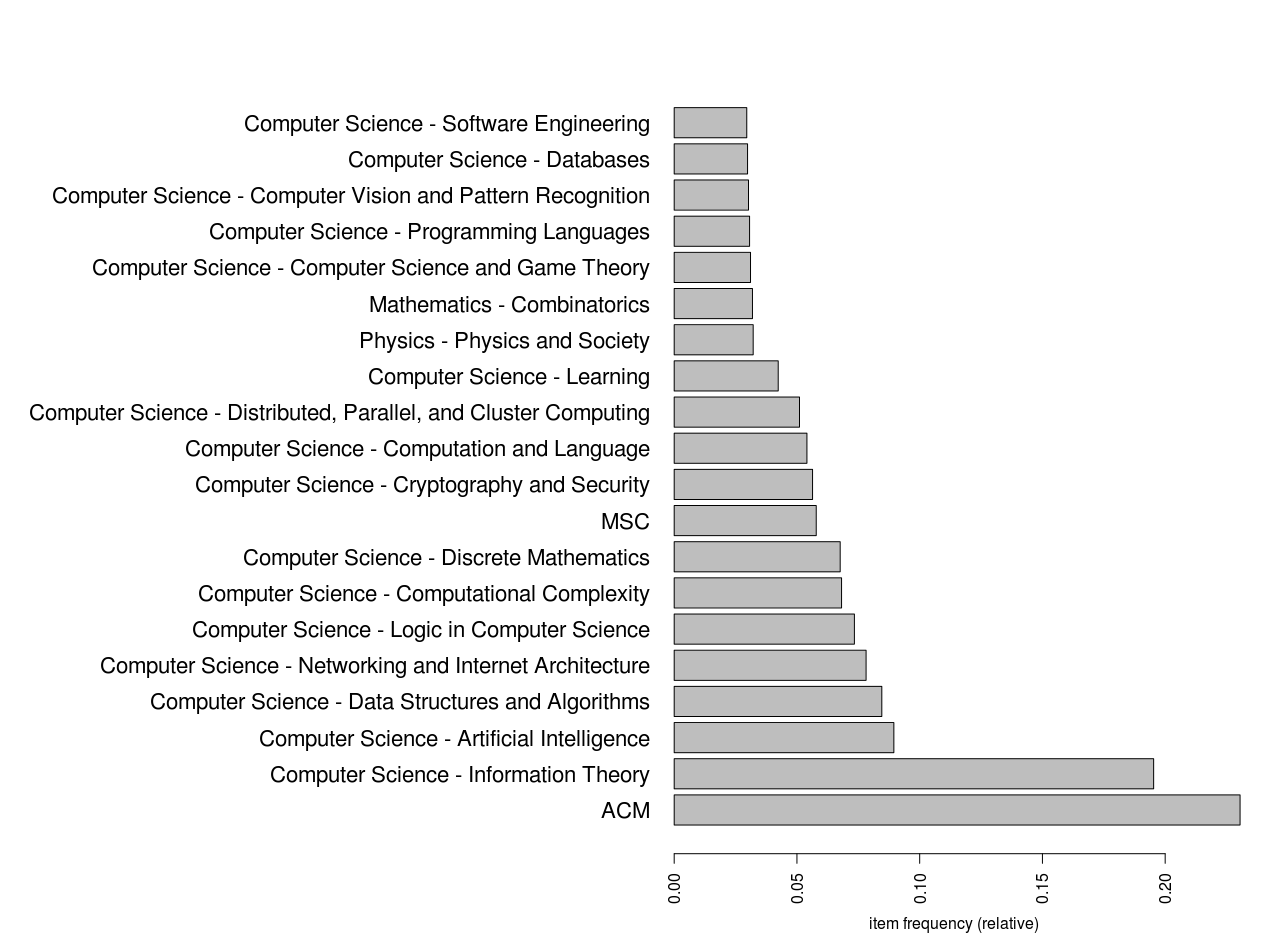
\includegraphics[scale=0.3]{../visual/horiCsFreq.png}
	\caption{Die 20 h�ufigsten Unterthemen bei Computer Science}
	\label{cs-freq}
\end{figure}
